\section{Electron + Hadronic Tau Channel}\label{sec:eTauhad}


\subsection{Event selection}\label{sec:et_selection}

%% Events must fire the single-electron trigger described in
%% Section~\ref{sec:triggers}.  We select reconstructed electrons
%% satisfying $p_T>35~\gev$, $\vert\eta\vert<2.1$, with a distance of
%% closest approach to the leading sum-$p_T^2$ primary vertex of less
%% than 0.045~cm (transvese) and 0.2~cm (longitudinal), passing the tight
%% working point of the e/$\gamma$ POG non-triggering MVA ID, having no
%% matched conversion nor missing hits, and within $\Delta R<0.5$ of the
%% HLT electron that fired the trigger.

Events must fire the single-electron trigger described in
Section~\ref{sec:triggers}.  We select reconstructed electrons
satisfying:
\begin{itemize}
  \item $p_T>35$ GeV and $\vert\eta\vert<2.1$
  \item distance of closest approach to the leading 
sum-$p_T^2$ primary vertex of less than 0.045~cm 
(transvese) and 0.2~cm (longitudinal)
  \item passing the tight working point of the e/$\gamma$ 
POG non-triggering MVA ID
  \item having no matched conversion nor missing hits
  \item within $\Delta R<0.5$ of the HLT electron that fired the trigger

\end{itemize}

%% Offline $\tauh$'s are required to have $p_{T}> 20~\gev$ and $\vert
%% \eta \vert < 2.1$, have a distance of closest approach to the leading
%% sum-$p_T^2$ primary vertex of less than 0.2~cm (longitudinal), pass
%% the new Decay Mode Finding requirement as either a 1-prong or 3-prong
%% $\tauh$, and pass the ``againstElectronVLooseMVA5'' and
%% ``againstMuonTight3'' identification requirements.
%% %The isolation used is ``CombinedIsolationDeltaBetaCorr3Hits.''

Offline $\tauh$'s are required to have:
\begin{itemize}
  \item $p_{T}> 20$ GeV and $\vert \eta \vert < 2.1$
  \item distance of closest approach to the leading
sum-$p_T^2$ primary vertex of less than 0.2~cm (longitudinal)
  \item pass the new Decay Mode Finding requirement as 
either a 1-prong or 3-prong $\tauh$
  \item pass the ``againstElectronVLooseMVA5'' and
``againstMuonTight3'' identification requirements
\end{itemize}

We build pairs of electrons and $\tauh$'s in which the electron and
$\tauh$ are separated by at least $\Delta R > 0.5$.  In events with
more than one such pair, we select the pair with the two most isolated
leptons, considering first the electron, and then the $\tauh$.  This
criterion was seen to have good efficiency for signal samples.  In the
rare case of multiple such pairs having identical isolation values,
the reconstructed $p_T$'s are considred, preferring higher values.

%% Following the ID, pt/eta cuts, trigger matching and $dR$ condition
%% there may still be more than one possible candidate pair. We resolve
%% this by selecting the pair with the two most isolated leptons, under
%% the assumption that this gives the highest efficiency for selecting
%% the correct pair in signal events.  The following is the logic for
%% comparing two pairs in a sorting algorithm that aims to resolve
%% ambiguous cases (e.g. multiple candidates with the same isolation
%% value).\par First prefer the pair with the most isolated candidate 1
%% (muon for $e\mu$ and electron for $e\tau$).\par If the isolation of
%% candidate 1 is the same in both pairs, prefer the pair with the
%% highest candidate 1 pt (for cases of genuinely the same isolation
%% value but different possible candidate 1).\par If the pt of candidate
%% 1 in both pairs is the same (likely because it's the same object) then
%% prefer the pair with the most isolated candidate 2 (tau for $e\tau$
%% and electron for $e\mu$).\par If the isolation of candidate 2 is the
%% same, prefer the pair with highest candidate 2 pt (for cases of
%% genuinely the same isolation value but different possible candidate
%% 2).

After a pair has been chosen for an event, we apply the following
isolation requirements on the leptons, for an event to enter the
signal region: electron relative isolation $<0.15$; \tauh isolation
``byTightCombinedIsolationDeltaBetaCorr3Hits.''  In order to keep the
different final states exclusive, an event is rejected if there is an
additional electron satisfying the above identification requirements
and with relative isolation $<0.3$, or a muon satisfying the
identification requirements described in
Section~\ref{sec:em_selection} with relative isolation $<0.3$.  To
reduce further possible di-electron events in the $\teth$ channel, an
event is rejected if there is an opposite-charge electron pair with
$\Delta R > 0.15$ in which both of the electrons satisfy $p_T >
15$ GeV, $\vert \eta \vert < 2.5$, the e/$\gamma$ POG ``veto'' ID,
and relative isolation $<0.3$.

As for the other channels, the signal region is defined as having
\begin{itemize}
  \item $\cos{\Delta \phi (e,\tau_{h})}<-0.95$
  \item $Q(e) \times Q(\tau_{h}) < 0 $
  \item $\ETslash>30$ GeV
  \item $P_{\zeta}- 3.1 \times P_{\zeta}^{vis} > -50$ GeV
  \item no jet with $p_T>30$ GeV tagged as a b-jet (CSV loose)
\end{itemize}

The distributions of these variables after preselection are shown in
Figures~\ref{fig:et_preselection_distributions1},~\ref{fig:et_preselection_distributions2},~\ref{fig:et_preselection_distributions3}.

\begin{figure}\centering
  \includegraphics[width=0.45\textwidth]{figures/et-em/kinematicDistributions_unblind/et_puweight_OS_1and3prong_met}
  \includegraphics[width=0.45\textwidth]{figures/et-em/kinematicDistributions_unblind/et_puweight_OS_1and3prong_Zeta} \\
  \includegraphics[width=0.45\textwidth]{figures/et-em/kinematicDistributions_unblind/et_puweight_OS_1and3prong_cosDPhi}
  \includegraphics[width=0.45\textwidth]{figures/et-em/kinematicDistributions_unblind/et_puweight_OS_1and3prong_nCSVL}
  \caption{\label{fig:et_preselection_distributions1} Distributions,
    after preselection, of the variables used for \teth signal
    selection: \ETslash (top left), ``$\zeta$'' (top right),
    $\cos{\Delta \phi (e,\tau_{h})}$ (bottom left), and $n_b$ (bottom
    right).}
\end{figure}

\begin{figure}\centering
  \includegraphics[width=0.45\textwidth]{figures/et-em/kinematicDistributions_unblind/et_puweight_OS_1and3prong_ePt}
  \includegraphics[width=0.45\textwidth]{figures/et-em/kinematicDistributions_unblind/et_puweight_OS_1and3prong_eEta} \\
  \includegraphics[width=0.45\textwidth]{figures/et-em/kinematicDistributions_unblind/et_puweight_OS_1and3prong_tPt}
  \includegraphics[width=0.45\textwidth]{figures/et-em/kinematicDistributions_unblind/et_puweight_OS_1and3prong_tEta}
  \caption{\label{fig:et_preselection_distributions2} Distributions,
    after \teth preselection, of electron \pt (top left), electron
    pseudo-rapidity (top right), $\tau$ \pt (bottom left), $\tau$
    pseudo-rapidity (bottom right).}
\end{figure}

\begin{figure}\centering
  \includegraphics[width=0.45\textwidth]{figures/et-em/kinematicDistributions_unblind/et_puweight_OS_1and3prong_mt}
  \includegraphics[width=0.45\textwidth]{figures/et-em/kinematicDistributions_unblind/et_puweight_OS_1and3prong_meff} \\
  \caption{\label{fig:et_preselection_distributions3} Distributions,
    after \teth preselection, of $m_{T}\left(e, \ETslash\right)$
    (left), $m\left(e, \tau, \ETslash\right)$ (right).}
\end{figure}

The distributions of these variables after preselection, and after
selection requirements on the other variables, are shown in
Figure~\ref{fig:et_nm1_distributions}.

\begin{figure}\centering
  \includegraphics[width=0.45\textwidth]{figures/et-em/n_1/et_MET}
  \includegraphics[width=0.45\textwidth]{figures/et-em/n_1/et_Zeta} \\
  \includegraphics[width=0.45\textwidth]{figures/et-em/n_1/et_cosDPhi}
  \includegraphics[width=0.45\textwidth]{figures/et-em/n_1/et_nb}
  \caption{\label{fig:et_nm1_distributions} Distributions of the
    variables used for \teth signal selection, after all other signal
    selection requirements on variables other than the one plotted:
    \ETslash (top left), ``$\zeta$'' (top right), $\cos{\Delta \phi
      (e,\tau_{h})}$ (bottom left), and $n_b$ (bottom right).}
\end{figure}

The Standard Model processes considered as backgrounds are Drell-Yan,
di-boson production, top quark single and pair production, W+jets
production, and QCD multi-jet production.

\subsection{Genuine dilepton events}

Studies of simulated events indicate that for Drell-Yan process, top
quark single and pair production, and di-boson production, the
reconstructed and selected electrons and hadronic taus are typically
associated with genuine simulated leptons.  The nominal expected event
rates are estimated by scaling the simulated samples by the best
available cross sections, listed in Table~\ref{tab:mc_samples}, and by
the integrated luminosity of the data samples.

\subsubsection{Drell-Yan process}
Due to large W+Jets and QCD contamination, as shown in the left panel of 
Figure~\ref{fig:et_dy_tt} with the following selections:
\begin{itemize}
  \item $\ETslash<30$ GeV;
  \item no jet with $p_T>30$ GeV tagged as a b-jet (CSV loose);
  \item \meffetau $<$ 200 GeV\quad,
\end{itemize}
we use the Drell-Yan rate systematic uncertainty (12\%) estimated from
the \tetm final state in~\ref{sec:em_DY}.

\subsubsection{$t\bar{t}$ and single top processes process}
For \teth, we estimate the \ttbar + single top production rate
systematics (8\%) using the \tetm final state, as described in
~\ref{sec:em_tt}, due to its higher top purity.  However we cross
check this in a \teth top-rich region, defined by the following
selections and shown in the right panel of Figure~\ref{fig:et_dy_tt}:
\begin{itemize}
  \item $\cos{\Delta \phi (e,\tau_{h})}<-0.95$
  \item $\ETslash>30$ GeV
  \item $P_{\zeta}- 3.1 \times P_{\zeta}^{vis} > -50$ GeV
  \item at least one jet with $p_T>30$ GeV tagged as a b-jet (CSV loose)
\end{itemize}
The $t\bar{t}$ + single top production rate systematics estimated to be:
\begin{equation}\label{eq:et_tt}
\text{$t\bar{t}$ + single top systematics} = \left| 1 - \frac{\text{$t\bar{t}$ + single top}}{\text{Data - other backgrounds}}\right| = 5\%\quad,
\end{equation}
in agreement with the estimate from \tetm.

\begin{figure}\centering
  \includegraphics[width=0.45\textwidth]{figures/et-em/Data_MC_Comparison/et_DY_Validation_Met_lessThan30_nCSVL_lessThan1_m_eff_lessThan200}
  \includegraphics[width=0.45\textwidth]{figures/et-em/eTauStudies/ttbar_check}
  %% \includegraphics[width=0.45\textwidth]{figures/et-em/Data_MC_Comparison/et_TT_Validation}
  \caption{\label{fig:et_dy_tt} Distributions of \meffetau. Left: validation region with $\ETslash<30$ GeV, $n_b = 0$ \meffetau $<$ 200 GeV.  Right: validation region with $n_b\geq1$.}
\end{figure}

\subsubsection{Di-boson process}
We take di-boson processes directly from simulation with a 15\% production uncertainty.

    
\subsection{QCD multi-jet background}\label{sec:etau_qcd}
For a given variable and binning, e.g. the effective mass variable
used for signal extraction, we construct a data-driven template for
the shape of the QCD multi-jet background, i.e. the processes lacking
prompt leptons.  Based on the charge of the final state and \tauh isolation,
we split the events into four regions shown in Figure~\ref{fig:ABCD} and 
described below:
\begin{itemize}
  \item A (Signal) Region: e and \tauh have opposite charge and \tauh pass "Tight" isolation requirement.
  \item B Region: e and \tauh have same charge and \tauh pass "Tight" isolation requirement.
  \item C Region: e and \tauh have opposite charge and \tauh pass anti-isolation requirement.
  \item D Region: e and \tauh have same charge and \tauh pass anti-isolation requirement.
\end{itemize}

\begin{figure}\centering
  \includegraphics[width=0.45\textwidth]{figures/et-em/figs/ABCD}
  \caption{\label{fig:ABCD} QCD estimation and validation strategy for the \teth channel.}
\end{figure}
In each region (B, C, D), QCD events are estimated by subtracting events
with genuine leptons (estimated by simulation) bin-by-bin from data.
QCD events are assumed to be charge blind, thus, the amount of QCD events in region B should be 
comparable to that of in the signal region. However, with the freedom to define the
anti-isolation region, we choose an anti-isolation definition such
that there are much more QCD in region C compared to the signal region. 
Taking the QCD shape from region C will provide us 
a much smoother template for QCD estimation.

Hence, QCD events in the signal region are estimated with the shape from region C 
and multiplying a scale factor derived from regions B and D. The factor is defined as:
\begin{equation}\label{eq:et_qcd_sf}
f_\mathrm{LT}^\mathrm{QCD} = \left(N_\mathrm{data}^\mathrm{B} - N_\mathrm{MC}^\mathrm{B}\right)
/ \left(N_\mathrm{data}^\mathrm{D} -
N_\mathrm{MC}^\mathrm{D}\right)\quad.
\end{equation}

This QCD estimation method is valid only if the QCD shape in
anti-isolated correctly models the QCD shape in the isolated
region. The check is done by comparing the observation and background
estimation in region B with the QCD shape taking from region D and
normalized to the QCD in region B.  An example of this test is shown
in the right panel of Figure~\ref{fig:et_sst} with the anti-isolation
definition as: \tauh isolation failing the "Tight" working point but
below 5.0 GeV.

With the freedom to define the \tauh anti-isolation region, before the 
signal region selections so there is enough statistics, we scan 
through different anti-isolation definitions as shown in Figure~\ref{fig:et_scans} 
where the x-axis labels the start of the anti-isolation region and the 
y-axis labels the end. With each anti-isolation definition, we perform 
the check mentioned above and calculate $\chi^2$ between observation 
and background estimation. The p-value of the $\chi^2$ tests for each 
anti-isolation definition is shown on the cells in the right panel 
of Figure~\ref{fig:et_scans}. The left panel of Figure~\ref{fig:et_scans} shows 
the same test but with $f_\mathrm{LT}^\mathrm{QCD}$ instead in each cell.

Based on the following criteria:
\begin{itemize}
  \item good results from $\chi^2$ test
  \item low "Loose-to-Tight" scale factor ($f_\mathrm{LT}^\mathrm{QCD}$) to ensure a smooth template
\end{itemize}

The range of isolation failing the tight working point, but below 5.0 GeV, was chosen as the
sideband with. After the signal region selection the "Loose-to-Tight" scale factor is estimated
to be: $0.13 \pm 0.02$ where an additional 15\% uncertainty is added to the QCD systematics 
on top of the bin-by-bin systematics.

\begin{figure}\centering
  \includegraphics[width=0.45\textwidth,page=68]{figures/et-em/antiIsolationScan/et_puweight_chi2_SS_123prong_antiIsoScan} %% et_SS_chi2Scan_SF
  \includegraphics[width=0.45\textwidth,page=67]{figures/et-em/antiIsolationScan/et_puweight_chi2_SS_123prong_antiIsoScan} %% et_SS_chi2Scan_p_value
  \caption{\label{fig:et_scans} \teth channel: scan of the range of
    relaxed isolation for the $\tau_h$.  Left: text within each bin
    gives the normalization factor applied to same-charge iso-relaxed
    events (``loose to tight'' factor); the color axis matches the
    right plot.  Right: $\chi^2$-probability of the agreement between
    the predicted and observed distributions of tightly-isolated
    same-charge events.}
\end{figure}

\begin{figure}\centering
  \includegraphics[width=0.45\textwidth,page=6]{figures/et-em/antiIsolationScan/et_puweight_chi2_SS_123prong_antiIsoScan} %% et_SST
  \caption{\label{fig:et_sst} The distribution of reconstructed parent
    mass, \meffetau, in the same-charge, tightly-isolated sample:
    \teth channel.}
\end{figure}

\subsection{W+jets background}
\label{sec:et_w_bkg_validation}

The simulated W+jets samples, especially at low HT, were not
generated with large MC statistics.  Using the samples directly would
have two disadvantages: (a) avoiding non-smooth templates in the
signal extraction would restrict somewhat the choice of signal
selection and binning; (b) the poorly sampled shapes degrade the
ability to validate the background estimates.  As a workaround, we use
a region of relaxed \tauh isolation to obtain the simulated shape:
\tauh isolation is required to fail the ``tight'' working point but be
less than $5$ GeV.  This shape template is then normalized to the
integrated MC yield when requiring tight \tauh isolation.

Figure~\ref{fig:et-w-shape} compares the direct and relaxed
predictions in the signal region and in the control region discussed
below.  It also shows the compatibility of the predicted shapes when
the isolation sideband is split into to regions: \tauh isolation
failing ``Tight'' working point but $<2.5$ GeV; $2.5$ GeV < \tauh
isolation < $5$ GeV.

\begin{figure}\centering
  \includegraphics[width=0.32\textwidth]{figures/et-em/WJetsClosureTest/highMETlowPZeta0BTag_m_withMET}
  %% \includegraphics[width=0.45\textwidth]{figures/et-em/WJetsClosureTest/highMETlowPZeta0BTag_mt}
  %% \includegraphics[width=0.45\textwidth]{figures/et-em/WJetsClosureTest/signalRegionSelection_m_withMET} \\
  \includegraphics[width=0.32\textwidth]{figures/et-em/bkgChecks/WJets_comparison_meff}
  \includegraphics[width=0.32\textwidth]{figures/et-em/eTauStudies/WJets_Tight_to_2p5_vs_2p5_5}
  \caption{\label{fig:et-w-shape} Left: comparison of the simulated
    distributions of \meffetau, using tight \tauh isolation and with
    relaxed \tauh isolation, in the control region described in
    Section~\ref{sec:et_w_bkg_validation}.  Center: analogous
    comparison for the signal region.  Right: comparison in the signal
    region of the ``tighter'' and ``looser'' halves of the sideband.}
\end{figure}

To evaluate the estimated background rate in a signal-depleted and
W-enriched region, we make the same requirements as for the signal
region, except require $p_{\zeta} - 3.1 p_{\zeta\mathrm{vis.}}<
-50$ GeV (i.e., inverted w.r.t. the signal selection), and allowing
any value of $\cos{\Delta\phi_{e\tauh}}$ (i.e., relaxed w.r.t. the
signal selection).  We then scan the W+jets event rate from 1.0 to
1.25, in steps of 0.05.  For each assumed rate, we redetermine the QCD
prediction in this control region.  Figure~\ref{fig:etau_w_sf} shows
the agreement between observations and background estimates at each
scan point.  A scale factor of $1.15\pm0.10$ gives the best agreement
in this control region.  The distribution of \meffetau in the
W-enriched control region, requiring also
$\cos{\Delta\phi_{e\tauh}}<-0.8$ (to be somewhat closer to the signal
region), is shown in Figure~\ref{fig:et_meff_flipped_pz}.

\begin{figure}\centering
  \includegraphics[width=0.3\textwidth,page=5]{figures/et-em/WJetsSFScan/et_puweight_OS_signalRegionReversePZeta_1and3prong_mt}
  \includegraphics[width=0.3\textwidth,page=6]{figures/et-em/WJetsSFScan/et_puweight_OS_signalRegionReversePZeta_1and3prong_mt}
  \includegraphics[width=0.3\textwidth,page=7]{figures/et-em/WJetsSFScan/et_puweight_OS_signalRegionReversePZeta_1and3prong_mt}\\
  \includegraphics[width=0.3\textwidth,page=8]{figures/et-em/WJetsSFScan/et_puweight_OS_signalRegionReversePZeta_1and3prong_mt}
  \includegraphics[width=0.3\textwidth,page=9]{figures/et-em/WJetsSFScan/et_puweight_OS_signalRegionReversePZeta_1and3prong_mt}
  \includegraphics[width=0.3\textwidth,page=10]{figures/et-em/WJetsSFScan/et_puweight_OS_signalRegionReversePZeta_1and3prong_mt}
  \caption{\label{fig:etau_w_sf} Distributions of
    $m_\mathrm{T}\left(e,\ETslash\right)$ obtained in the W-enriched
    control region, when scanning the W+jets event rate from 1.0 to
    1.25 times its nominal value, in steps of 0.05.  For each assumed
    W+jets event rate, the QCD prediction is determined anew using the
    procedure described in Section~\ref{sec:etau_qcd}.}
\end{figure}

\begin{figure}\centering
  \includegraphics[width=0.45\textwidth]{figures/et-em/Data_MC_Comparison/et_puweight_OS_signalRegionReversePZeta_1and3prong_lessThan-0p8}
  \caption{\label{fig:et_meff_flipped_pz} \teth channel: the
    distribution of reconstructed parent mass, \meffetau, in the
    W-validation region described in
    Section~\ref{sec:et_w_bkg_validation}.}
\end{figure}

\clearpage
\subsection{Overlays of observations and SM predictions}
\label{sec:et_overlays}

The expected SM event yields in the signal region are shown in
Figure~\ref{fig:etau_sm_template_and_mt}.
\begin{figure}\centering
  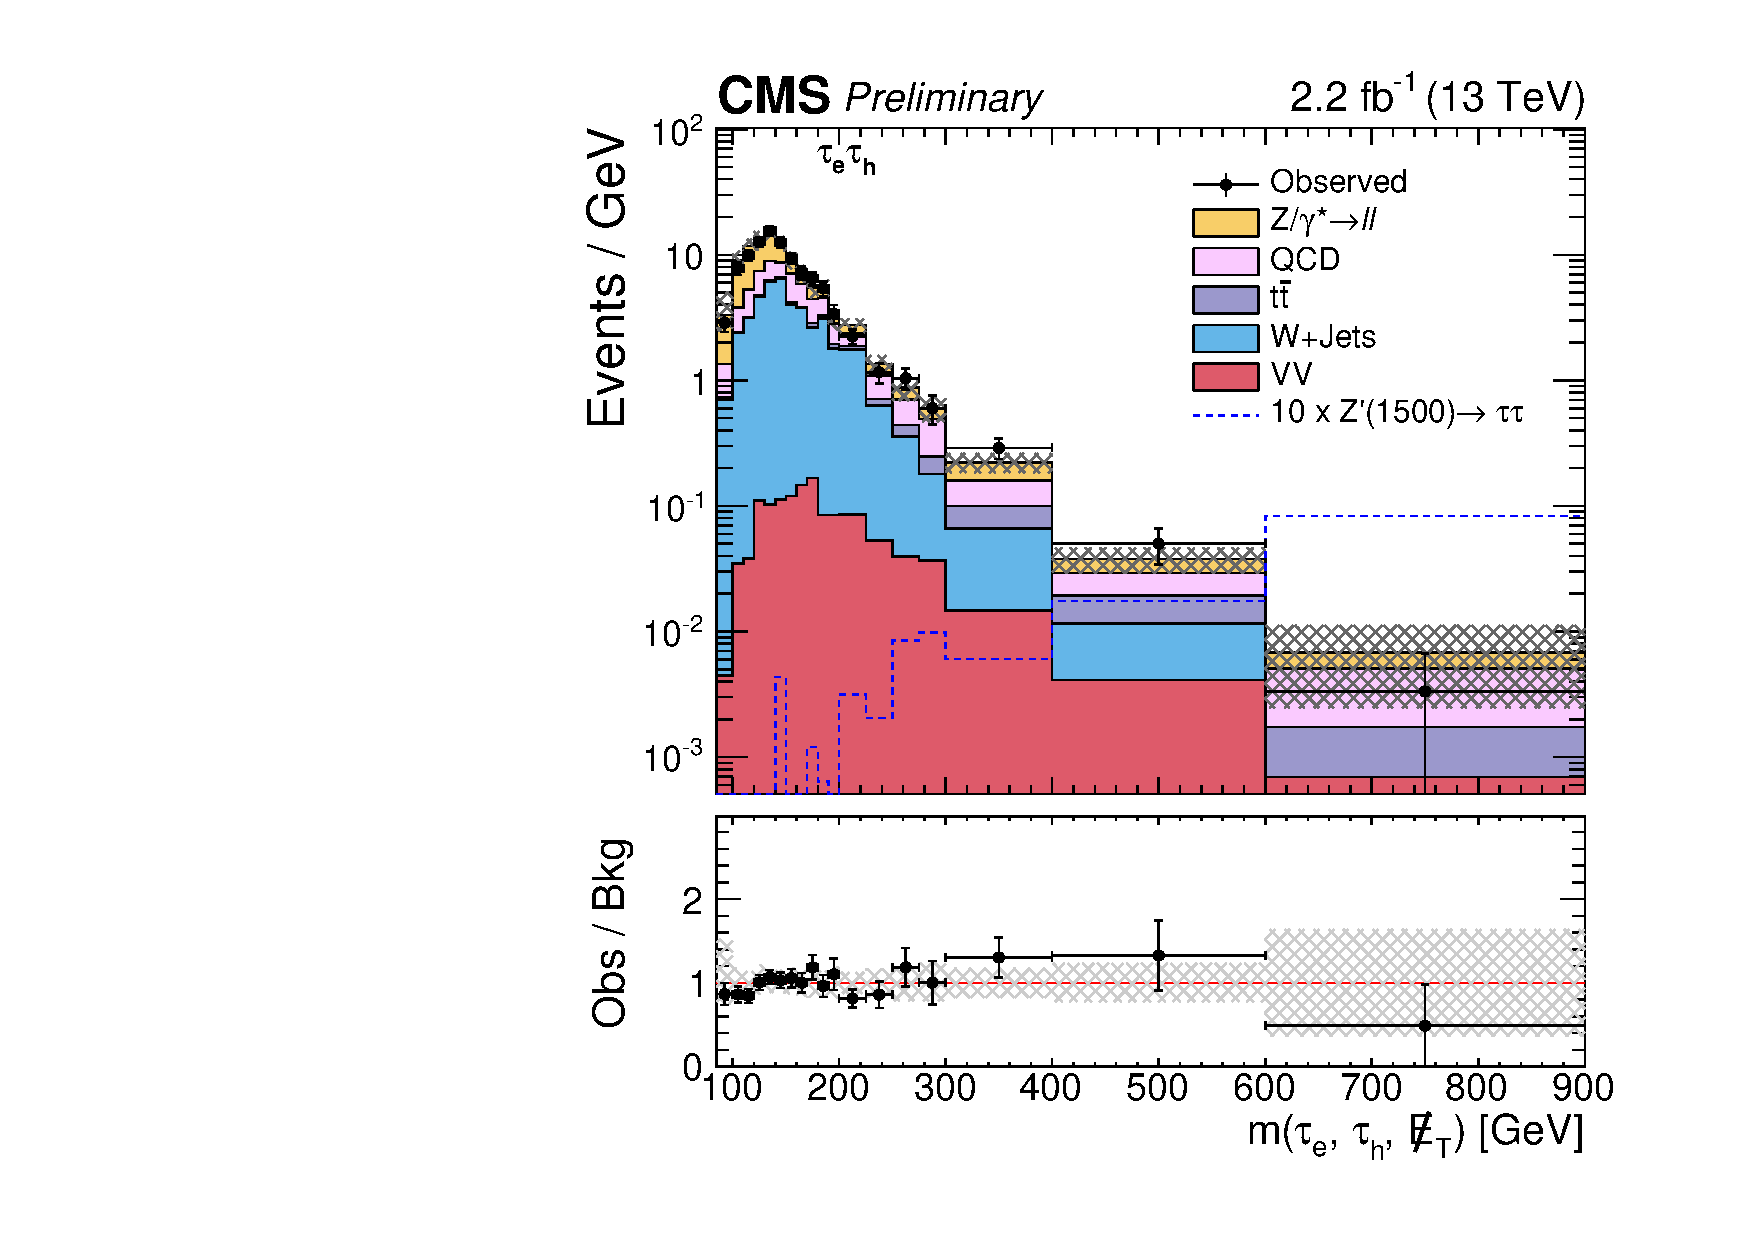
\includegraphics[width=0.45\textwidth]{figures/bkgTemplate_ZPrime1500_et}
  \includegraphics[width=0.45\textwidth]{figures/et-em/kinematicDistributions_unblind/et_puweight_OS_signalRegion_1and3prong_mt}
  \caption{\label{fig:etau_sm_template_and_mt} Left: predicted
    background yields and observed event yields in the \teth channel
    after signal selection.  Right: the distribution of transverse
    mass.}
\end{figure}

Distributions of \pt and $\eta$ are shown in Figure~\ref{fig:etau_sr_pt_eta}.
\begin{figure}\centering
  \includegraphics[width=0.45\textwidth]{figures/et-em/kinematicDistributions_unblind/et_puweight_OS_signalRegion_1and3prong_ePt}
  \includegraphics[width=0.45\textwidth]{figures/et-em/kinematicDistributions_unblind/et_puweight_OS_signalRegion_1and3prong_eEta} \\
  \includegraphics[width=0.45\textwidth]{figures/et-em/kinematicDistributions_unblind/et_puweight_OS_signalRegion_1and3prong_tPt}
  \includegraphics[width=0.45\textwidth]{figures/et-em/kinematicDistributions_unblind/et_puweight_OS_signalRegion_1and3prong_tEta}
  \caption{\label{fig:etau_sr_pt_eta} Distributions, after \teth final
    selection, of electron \pt (top left), electron pseudo-rapidity
    (top right), $\tau$ \pt (bottom left), $\tau$ pseudo-rapidity
    (bottom right).}
\end{figure}

%% figures/et-em/kinematicDistributions_unblind/et_puweight_OS_signalRegion_1and3prong_tEta_300_mEff_600.pdf
%% figures/et-em/kinematicDistributions_unblind/et_puweight_OS_signalRegion_1prong_tPt.pdf
%% figures/et-em/kinematicDistributions_unblind/et_puweight_OS_signalRegion_3prong_tPt.pdf
%% figures/et-em/kinematicDistributions_unblind/et_puweight_SS_signalRegion_1prong_tPt.pdf
%% figures/et-em/kinematicDistributions_unblind/et_puweight_SS_signalRegion_3prong_tPt.pdf
%% figures/et-em/kinematicDistributions_unblind/et_puweight_OS_signalRegion_2prong_tPt.pdf


\subsection{Post-unblinding: further checks of the backgrounds}
\label{sec:et_bkg_validation}

%% \begin{figure}\centering
%%   \includegraphics[width=0.45\textwidth]{figures/et-em/eTauStudies/excessCloseUp}
%%   \caption{\label{fig:closeUp} The distributions of
%%     reconstructed parent mass between 300 to 600 GeV, \teth channel:
%%     \meffetau.}
%% \end{figure}

%% The background composition for \meffetau in region [300, 600] is shown
%% in Figure~\ref{fig:closeUp}. As shown, the dominating background in
%% this region is W+Jets, consisting of around 55\% of the total
%% background, followed by QCD accounting for 19\% and $t\bar{t}$
%% accounting for 16\% of the total background.

\subsubsection{Checks of MC-based W+Jets}
Based on $m_T$ distribution shown in
Figure~\ref{fig:etau_sm_template_and_mt}, we require $60~\text{GeV} <
m_T < 120~\text{GeV}$ to compare data v.s estimated background in a
W+Jets rich region. Figure~\ref{fig:60_mT_120} shows that the W+Jets
shape estimated from the relaxed \tauh isolation region provides a
smoother template and agrees better with observations.
\begin{figure}\centering
  \includegraphics[width=0.45\textwidth]{figures/et-em/eTauStudies/WJets_non_Iso_60_mt_120}
  \includegraphics[width=0.45\textwidth]{figures/et-em/eTauStudies/WJets_iso_60_mt_120}
  \caption{\label{fig:60_mT_120} \teth channel, in the signal region,
    requiring also $60~\text{GeV} < m_T < 120~\text{GeV}$.  Left: The
    distributions of \meffetau with W+Jets shape estimated from
    relaxed \tauh isolation region. Right: The distributions of
    \meffetau with W+Jets shape estimated from tight \tauh isolation
    region.}
\end{figure}

%% A direct comparison of the W+Jets tight and sideband shapes, in three
%% slices of $m_T$, is shown in Figure~\ref{fig:et_WJets_mT}. When
%% $60~\gev < m_T < 120~\gev$, there appears to be a significant upward
%% fluctuation of W+Jets in the tight \tauh isolation region for
%% \meffetau regions of [300, 600].  In the other two slices of $m_T$,
%% the isolated and anti-isolated shapes look compatible within
%% statistics.

%% \begin{figure}\centering
%%   \includegraphics[width=0.32\textwidth]{figures/et-em/eTauStudies/WJets_iso_vs_non-Iso_mt_60}
%%   \includegraphics[width=0.32\textwidth]{figures/et-em/eTauStudies/WJets_iso_vs_non-Iso_60_mt_120}
%%   \includegraphics[width=0.32\textwidth]{figures/et-em/eTauStudies/WJets_iso_vs_non-Iso_120_mt}

%%   \caption{\label{fig:et_WJets_mT} \teth channel: comparison of the
%%     simulated W+jets distributions of \meffetau in the signal region,
%%     using tight \tauh isolation (red) or the \tauh isolation sideband
%%     from ``tight'' to 5\gev (blue).  Left: $m_T < 60\gev$. Center:
%%     $60\gev < m_T < 120\gev$.  Right: $120\gev < m_T$.}
%% \end{figure}

%% For $m_T > 120~\text{GeV}$, W+Jets shape comparisons and distributions
%% of \meffetau are shown in Figure~\ref{fig:120_mT}.  Due to low
%% statistics, it is difficult to conclude if there are any excess in
%% \meffetau regions [300, 600]. Overall, W+Jets shape estimated from the
%% relaxed \tauh isolation region agrees better with observations.

%% \begin{figure}\centering
%%   \includegraphics[width=0.45\textwidth]{figures/et-em/eTauStudies/WJets_non_Iso_120_mt}
%%   \includegraphics[width=0.45\textwidth]{figures/et-em/eTauStudies/WJets_iso_120_mt}
%%   \caption{\label{fig:120_mT} \teth channel, in the signal region,
%%     requiring also $m_T > 120~\gev$: Left: the distributions of
%%     \meffetau with W+Jets shape estimated from relaxed \tauh isolation
%%     region. Right: the distributions of \meffetau with W+Jets shape
%%     estimated from tight \tauh isolation region.}
%% \end{figure}

%% In the signal rich region, with $m_T < 60~\text{GeV}$,
%% Figure~\ref{fig:mT_60} shows that the excess seen in the high
%% \meffetau region cannot be explained by W+Jets MC shape variations
%% between relaxed and tight \tauh isolation regions.
%% \begin{figure}\centering
%%   \includegraphics[width=0.45\textwidth]{figures/et-em/eTauStudies/WJets_non_Iso_mt_60}
%%   \includegraphics[width=0.45\textwidth]{figures/et-em/eTauStudies/WJets_iso_mt_60}
%%   \caption{\label{fig:mT_60} \teth channel, in the signal region
%%     requiring also $m_T < 60~\gev$.  Left: The distributions of
%%     \meffetau with W+Jets shape estimated from relaxed \tauh isolation
%%     region. Right: The distributions of reconstructed parent mass with
%%     W+Jets shape estimated from tight \tauh isolation region. \teth
%%     channel}
%% \end{figure}

For the \teth channel, 2-prong \tauh's were rejected due low signal
presence and high W+Jets and QCD contamination.  Hence, 2-prong
\tauh's provide a testing group for the background estimation
methods. As shown in Figure~\ref{fig:et_2prong} there is a good
agreement between observations and estimated background.

\begin{figure}\centering
  \includegraphics[width=0.45\textwidth]{figures/et-em/eTauStudies/2prong}
  \caption{\label{fig:et_2prong} In the signal region, but requiring
    2-prong \tauh's: the distribution of reconstructed parent mass,
    \meffetau, with W+Jets shape estimated from relaxed \tauh
    isolation region.}
\end{figure}

\subsubsection{Data-driven W+jets checks}
Similar to the \tmth channel, by requesting e and \tauh to have opposite charge, 
we have the following four regions:
\begin{itemize}
  \item A (Signal) Region: pass "$\zeta$" and "$\cos\Delta\phi$" and \tauh pass "Tight" isolation requirement.
  \item B Region: fail "$\zeta$" or "$\cos\Delta\phi$" and \tauh pass "Tight" isolation requirement.
  \item C Region: pass "$\zeta$" and "$\cos\Delta\phi$" and \tauh pass anti-isolation requirement.
  \item D Region: fail "$\zeta$" or "$\cos\Delta\phi$" and \tauh pass anti-isolation requirement.
\end{itemize}
where the W+jets in the signal region is estimated from region C 
by subtracting all other background from data and multiplying a 
scale factor estimated among region B and D.
\begin{equation}\label{eq:et_data_WJets}
N^{\text{signal}}_{\text{W+jets}} = N^{\text{C}}_{\text{data - other bkg}} \times \frac{N^{\text{B}}_{\text{data - other bkgs}}}{N^{\text{D}}_{\text{data - other bkg}}}
\end{equation}

QCD in each region is estimated from data by inverting the charge
requirement.  Thus, we have four more regions A', B', C' and D' with
similar requirements as ABCD but requesting e and \tauh to have the
same charge. Hence, QCD in B, C and D regions are estimated in the
following way:
\begin{itemize}
  \item QCD in B Region: shape taken from data - all MC bkg (including W+jets MC) in D' region. 
Yield normalized to data - all MC bkg (including W+jets MC) in D region with a "SStoOS" scale 
factor of 1.07 $\pm$ 0.05 estimated from the \thth channel.
  \item QCD in C Region: shape taken from data - all MC bkg (including W+jets MC) in C' region. 
Yield normalized to data - all MC bkg (including W+jets MC) in C region
  \item QCD in D Region: shape taken from data - all MC bkg (including W+jets MC) in D' region. 
Yield normalized to data - all MC bkg (including W+jets MC) in D region.
\end{itemize}

The right panel of Figure~\ref{fig:dataDrivenWJets} shows the observation and background 
estimation comparisons with the data-driven W+jets and QCD estimations mentioned above. Compared 
with the MC W+jets estimation on the left panel, we see negligible difference between the 
two.

\begin{figure}\centering
  \includegraphics[width=0.45\textwidth]{figures/et-em/eTauStudies/et_puweight_OS_signalRegion_MCWJets_1and3prong}
  \includegraphics[width=0.45\textwidth]{figures/et-em/eTauStudies/et_puweight_OS_signalRegion_dataDrivenWJets_1and3prong}
  \caption{\label{fig:dataDrivenWJets} Left: W+jets shape and yield from simulation
    Right: Data-driven W+jets estimation \teth
    channel: \meffetau}
\end{figure}


